\documentclass[fleqn,10pt]{physiome}
% Use option lineno for line numbers
\usepackage[font=small,labelfont=bf,
   justification=justified,
   format=plain]{caption} % 'format=plain' avoids hanging indentation
\usepackage{appendix}
\usepackage{physics}
\usepackage{xcolor}
\usepackage{float}
\usepackage[section]{placeins}
\definecolor{blueheader}{RGB}{58, 110, 143}
\articletype{Original}
%% Choose from Original, Retrospective, Review, Letter
\newcommand{\note}[1]{}
\renewcommand{\note}[1]{{\color{red} \textit{[{#1}]}}}

\title{Reproducibility Study of Computational Modelling of Glucose Uptake by SGLT1 and GLUT2 in the Enterocyte}

\author[1]{Nima Afshar}
\author[1]{Soroush Safaei}
\author[1]{David P. Nickerson}
\author[1]{Peter J. Hunter}
\author[1,2][vinod.suresh@auckland.ac.nz]{Vinod Suresh}

\affil[1]{Auckland Bioengineering Institute, University of Auckland, Auckland, New Zealand}
\affil[2]{Department of Engineering Science, University of Auckland, Auckland, New Zealand}

%% The following lines can be omitted when submitting;
%% information will be added by editors
\publicationdate{19/01/2023}
\editor{Karin Lundengård}
\curator{Weiwei Ai}
\submitteddate{11 Aug 2022}
\accepteddate{11 Dec 2022}
\citethisas{Afshar et al. (2023) Reproducibility Study of Computational Modelling of Glucose Uptake by SGLT1 and GLUT2 in the Enterocyte. Physiome.}{10.36903/physiome.21708179}
\begin{document}

\maketitle

\begin{abstract}
\cite{afshar2021computational} generated a computational model of non-isotonic glucose uptake by small intestinal epithelial cells. The model incorporates apical uptake via SGLT1 and GLUT2, basolateral efflux into the blood via GLUT2 and cellular volume changes in response to non-isotonic conditions. The results explain more about the role of apical GLUT2 in intestinal cell glucose absorption. Here, we used the CellML file provided by the model authors, together with SED-ML files and Python scripts, to demonstrate the reproduction of the figures in the original paper by using the associated model.
\end{abstract}

\keywords{Physiome; CellML; OpenCOR; reproducibility; glucose uptake; water transport; SGLT1; GLUT2; ion channels.}

\primarypubs[10.36903/physiome.21708179]{references}{afshar2021computational}

\section{Introduction}

Glucose absorption through epithelial cells in the small intestine is known to be the main source of energy generation in humans and other species. Despite the number of investigations in recent decades \citep{mccance1930comparative, wertheimer1934phloridzinwirkung}, the absorption mechanism and transporters involved under different conditions and in different species are still not clear enough and are being debated \citep{karasov2017}.

% For many years the only known pathway for glucose absorption in the intestinal cell was SGLT1 \citep{ferraris2001dietary}, which works perfectly when the luminal glucose concentration is low, however SLGT1 is saturated around $30$ mM whereas glucose absorption is not saturated even at $100$ mM of extracellular glucose \citep{kellett2000diffusive} which is more similar to simple diffusion \citep{fullerton1956absorption, debnam1975experimental}. One of the theories to explain the glucose diffusion was paracellular flow or solvent drag which was based on the absorption of glucose during the water absorption process \citep{fullerton1956absorption, pappenheimer1987physiological}, However, multiple studies showed that paracellular glucose absorption is insignificant and negligible \citep{ferraris1990luminal, ferraris1997regulation, lane1999paracellular}. Other study detected the presence of GLUT2 in the brush border membrane of diabetic rat \citep{corpe1996regulation} which initiated the other theory based on translocation of GLUT2 to the apical membrane of epithelial cell in the presence of high luminal glucose concentration \citep{kellett2000diffusive, au2002rapid, affleck2003immunocytochemical, gouyon2003simple}. Imaging studies have also shown translocation of GLUT2 transporter into apical membrane from basolateral membrane of the cell as a response to high glucose accumulation in the lumen \citep{Cohen2014}. Mathematical models can be very helpful in order to study glucose uptake under different circumstances and investigate different theories.

% A model of sodium/potassium homeostasis in the enterocyte during SGLT1-mediated absorption was developed in 2014 \citet{thorsen2014transepithelial} however, it was limited to iso-osmotic conditions and did not have all the transporters. In their model SGLT1 was the only responsible transporter for glucose absorption in the apical membrane. Glucose transport can change the osmolarity leading to changes in water transport and cell volume. Cell volume can swell or shrink by gaining and losing water respectively \citep{zeuthen2007water}.  

% Another mathematical model explored the role of apical GLUT2 in glucose absorption as well as water transport and cell volume regulation. In their model SGLT1 and GLUT2 are the main transporters involved in glucose absorption in the apical and basolateral membrane and apical GLUT2 acts as an osmoregulator \citep{naftalin2016computer}. 


In 2019, Afshar et al. implemented a glucose absorption model in the enterocyte that contains all responsible transporters and was built using the CellML framework. Their model was used to study the role of SGLT1 and apical GLUT2, especially in the presence of a high glucose concentration in the intestinal lumen \citep{afshar2019computational}. They later extended their model to a non-isotonic glucose uptake considering water transport and changes in cell volume during the absorption process \citep{afshar2021computational}. 

A CellML version \citep{cuellar2003overview} of their model can be found in the Physiome Model Repository \citep{yu_physiome_2011}. However, the CellML file itself is not sufficient to reproduce all the predictions presented in the primary article. Therefore, some SED-ML files \citep{waltemath2011reproducible} and Python scripts were created and used with the aforementioned CellML file to reproduce the main results of \citet{afshar2021computational}. No modifications were made to the mathematical equations or parameters of the CellML file. All the equations and parameters can be found in the original paper. In the primary article, a validated computational model was proposed. The main goal of this paper is to show that the figures in the primary paper can be reproduced by using the correlated model in the PMR. Here, we introduce a quick instruction to reproduce each figure in the original paper.


\section{Model description}
The model contains several relevant transporters on either side of the intestinal cell, which has three different compartments (mucosal or intestinal lumen, cell and blood or serosal). The movement of transcellular and paracellular water was based on the osmolarity difference between the two compartments involved, leading to changes in cell volume. Ions and glucose move into and out of the cell through specific transporters. Using the mathematical model, it is possible to predict membrane potentials, intracellular concentrations of glucose and electrolytes (Na$^+$, K$^+$, HCO$_3^-$, Cl$^-$), and the fluxes of these species. All the equations for ions' fluxes and concentrations are described in the supplementary material in the primary paper. 

The model was developed in CellML. Simulations were run until the concentration and fluxes reached steady state. A CellML encoded version of the model is available at \url{https://models.physiomeproject.org/workspace/841}. The simulation results presented here were produced using the 2021-10-05 snapshot of OpenCOR \citep{garny2015opencor} together with various Python scripts that rely on a SED-ML file to configure (the solver to use, the duration of the simulation, the model parameters to track, etc.) and run a given simulation using the model encoded in CellML. Python scripts are also used to generate figures using Matplotlib \citep{Hunter:2007}. All CellML, SED-ML and Python scripts can be found in \url{https://models.physiomeproject.org/workspace/840}.

\section{Model results}

\begin{figure}[htb]
\centering
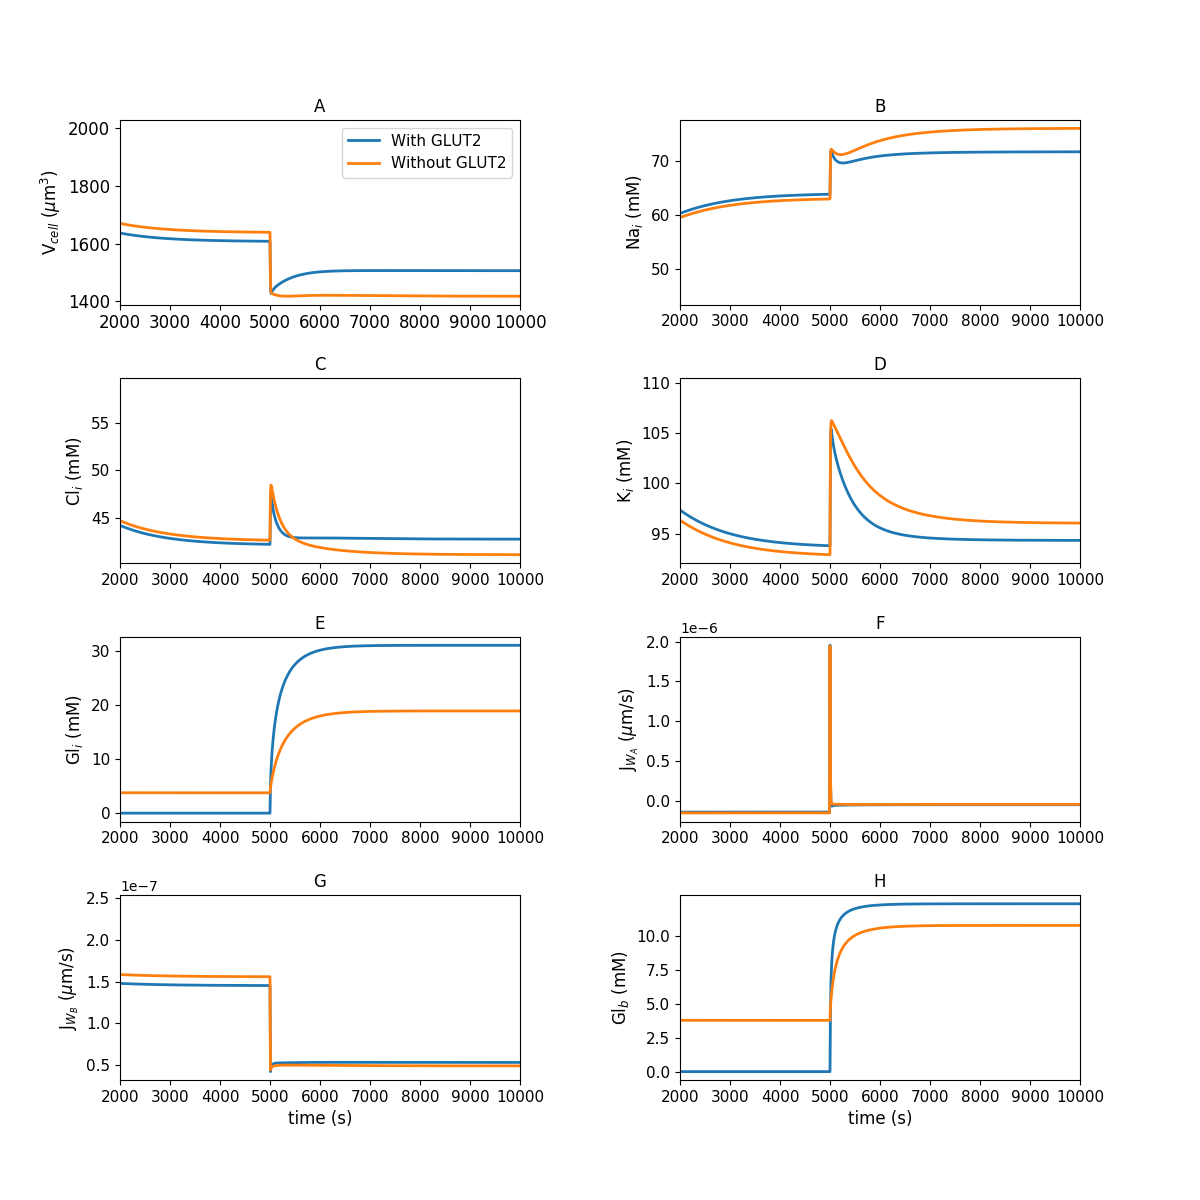
\includegraphics[width=0.9\linewidth]{Figure01}
\caption{Model behaviour in the absence of luminal glucose ($t<5,000$ s) and following a step change to $50$ mM luminal glucose ($5,000 \leq t<10,000$ s) of the simulation. (A) cell volume; (B) intracellular concentrations of sodium; (C) chloride; (D) potassium; (E) glucose; (F,G) apical and basolateral water flux; (H) blood glucose. This figure corresponds to Figure 3 in the primary paper and can be reproduced using \href{https://models.physiomeproject.org/workspace/840/rawfile/bc7a5ac43ddbd15d234e66d8cb17df8388d80064/Figure01.py}{Figure01.py}.}
\label{Figure1}
\end{figure}

\begin{figure}[htb]
\centering
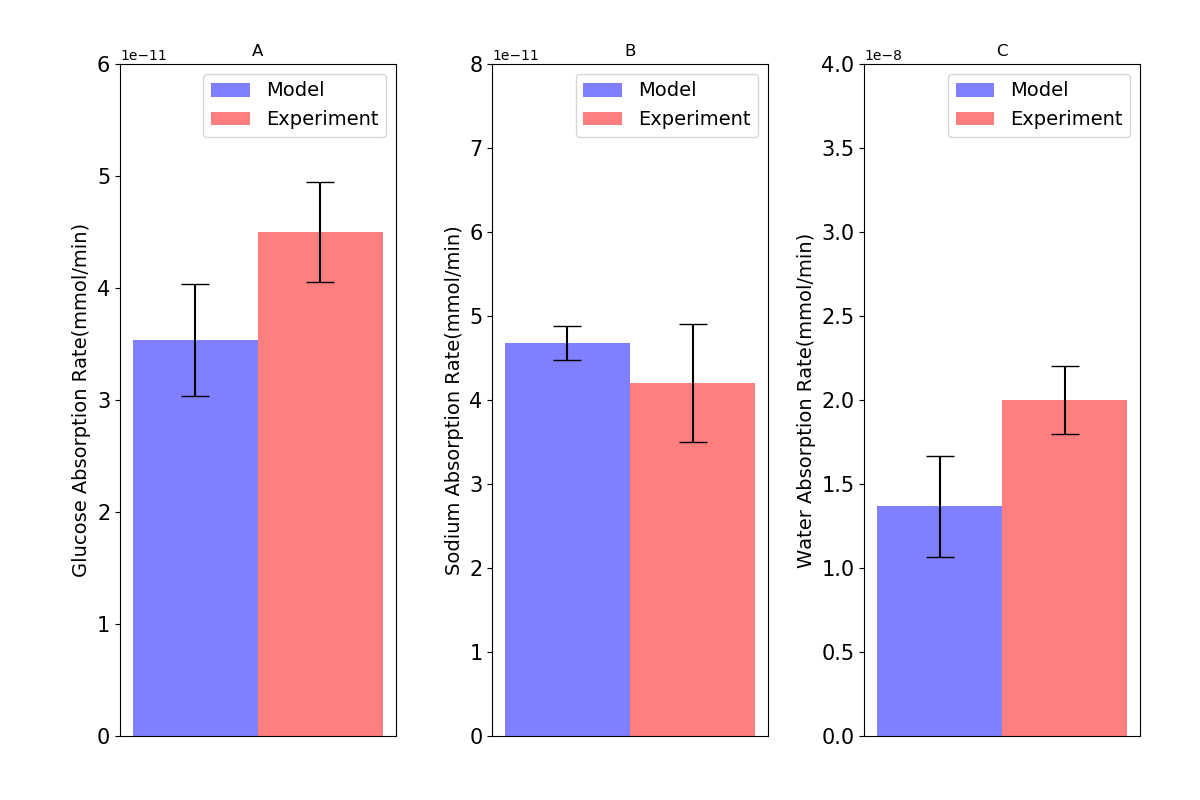
\includegraphics[width=0.9\linewidth]{Figure02}
\caption{Absorption rates of (A) glucose; (B) sodium; and (C) water through the cell in comparison with intestinal loop data. Error bars in the model represent different values for inlet blood flow. Experimental bars are mean $\pm$ SE with $6$ tests. This figure corresponds to Figure 4 in the primary paper and can be reproduced using \href{https://models.physiomeproject.org/workspace/840/rawfile/bc7a5ac43ddbd15d234e66d8cb17df8388d80064/Figure02.py}{Figure02.py}.}
\label{Figure2}
\end{figure}

\begin{figure}[htb]
\centering
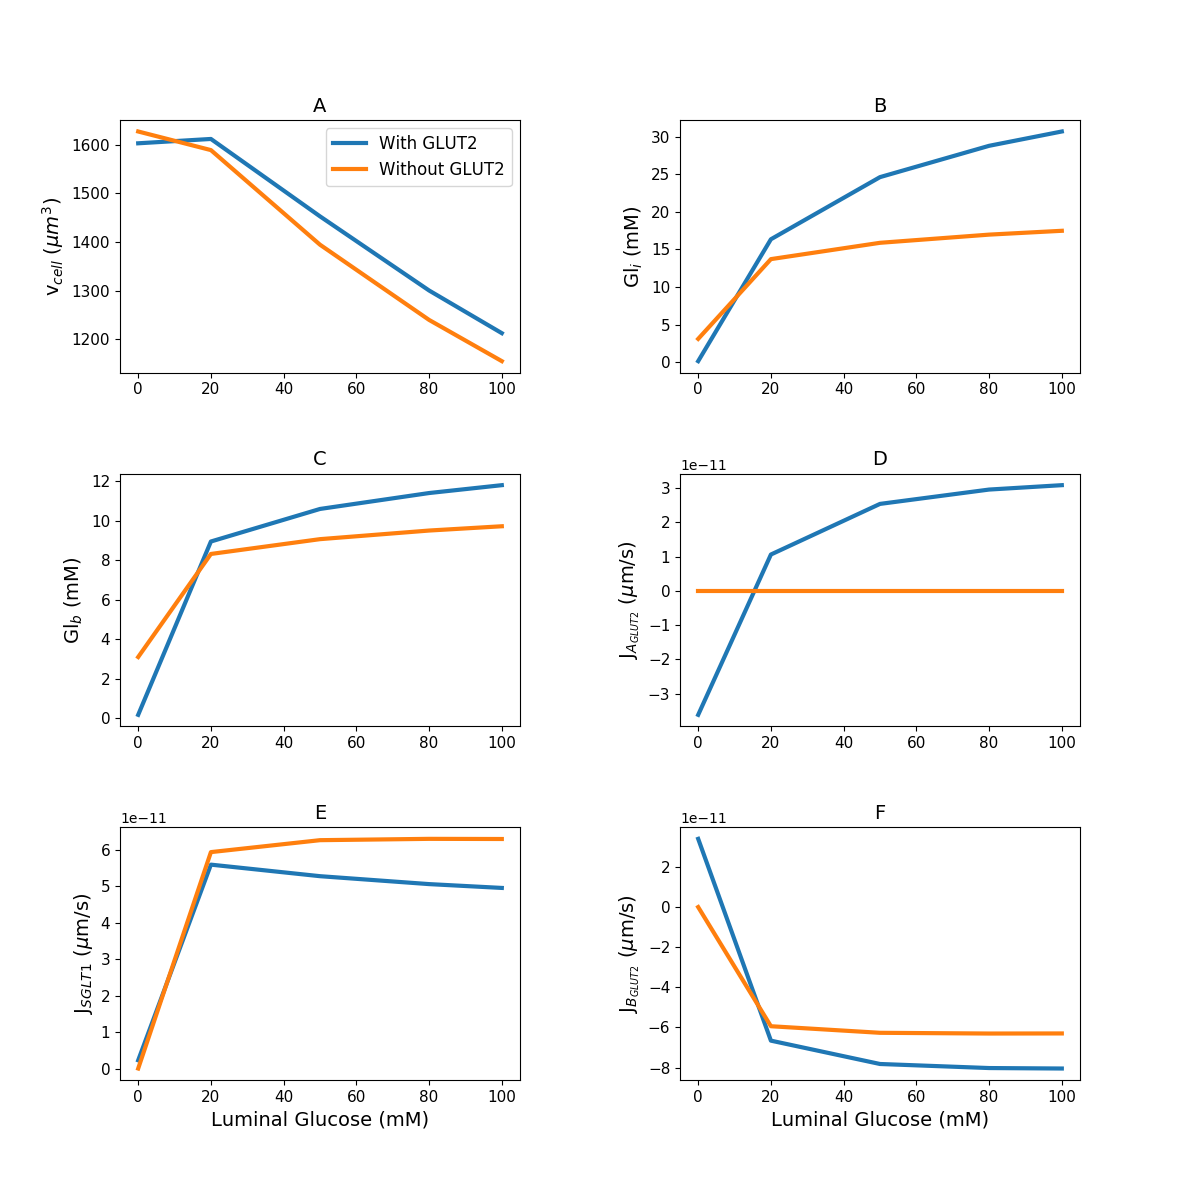
\includegraphics[width=0.9\linewidth]{Figure03}
\caption{Model response to different luminal glucose concentration. (A) Cell volume; (B) intracellular glucose; (C) blood glucose; (D) apical GLUT2 flux; (E) SGLT1 flux; (F) basolateral GLUT2 flux. The simulation was run under five different luminal glucose concentration ($0$, $20$, $50$, $80$, and $100$ mM). Simulation parameters: number of apical GLUT2 $=10^8$, number of basolateral GLUT2 $=2\times10^8$, number of SGLT1 $=3\times10^7$, inflow blood glucose $=4$ mM, inlet blood flow rate $=10^{-17}$ m${^3}$/s, and blood volume $=10^{-16}$ m$^3$. This figure corresponds to Figure 5 in the primary paper and can be reproduced using \href{https://models.physiomeproject.org/workspace/840/rawfile/bc7a5ac43ddbd15d234e66d8cb17df8388d80064/Figure03.py}{Figure03.py}.}
\label{Figure3}
\end{figure}

\begin{figure}[htb]
\centering
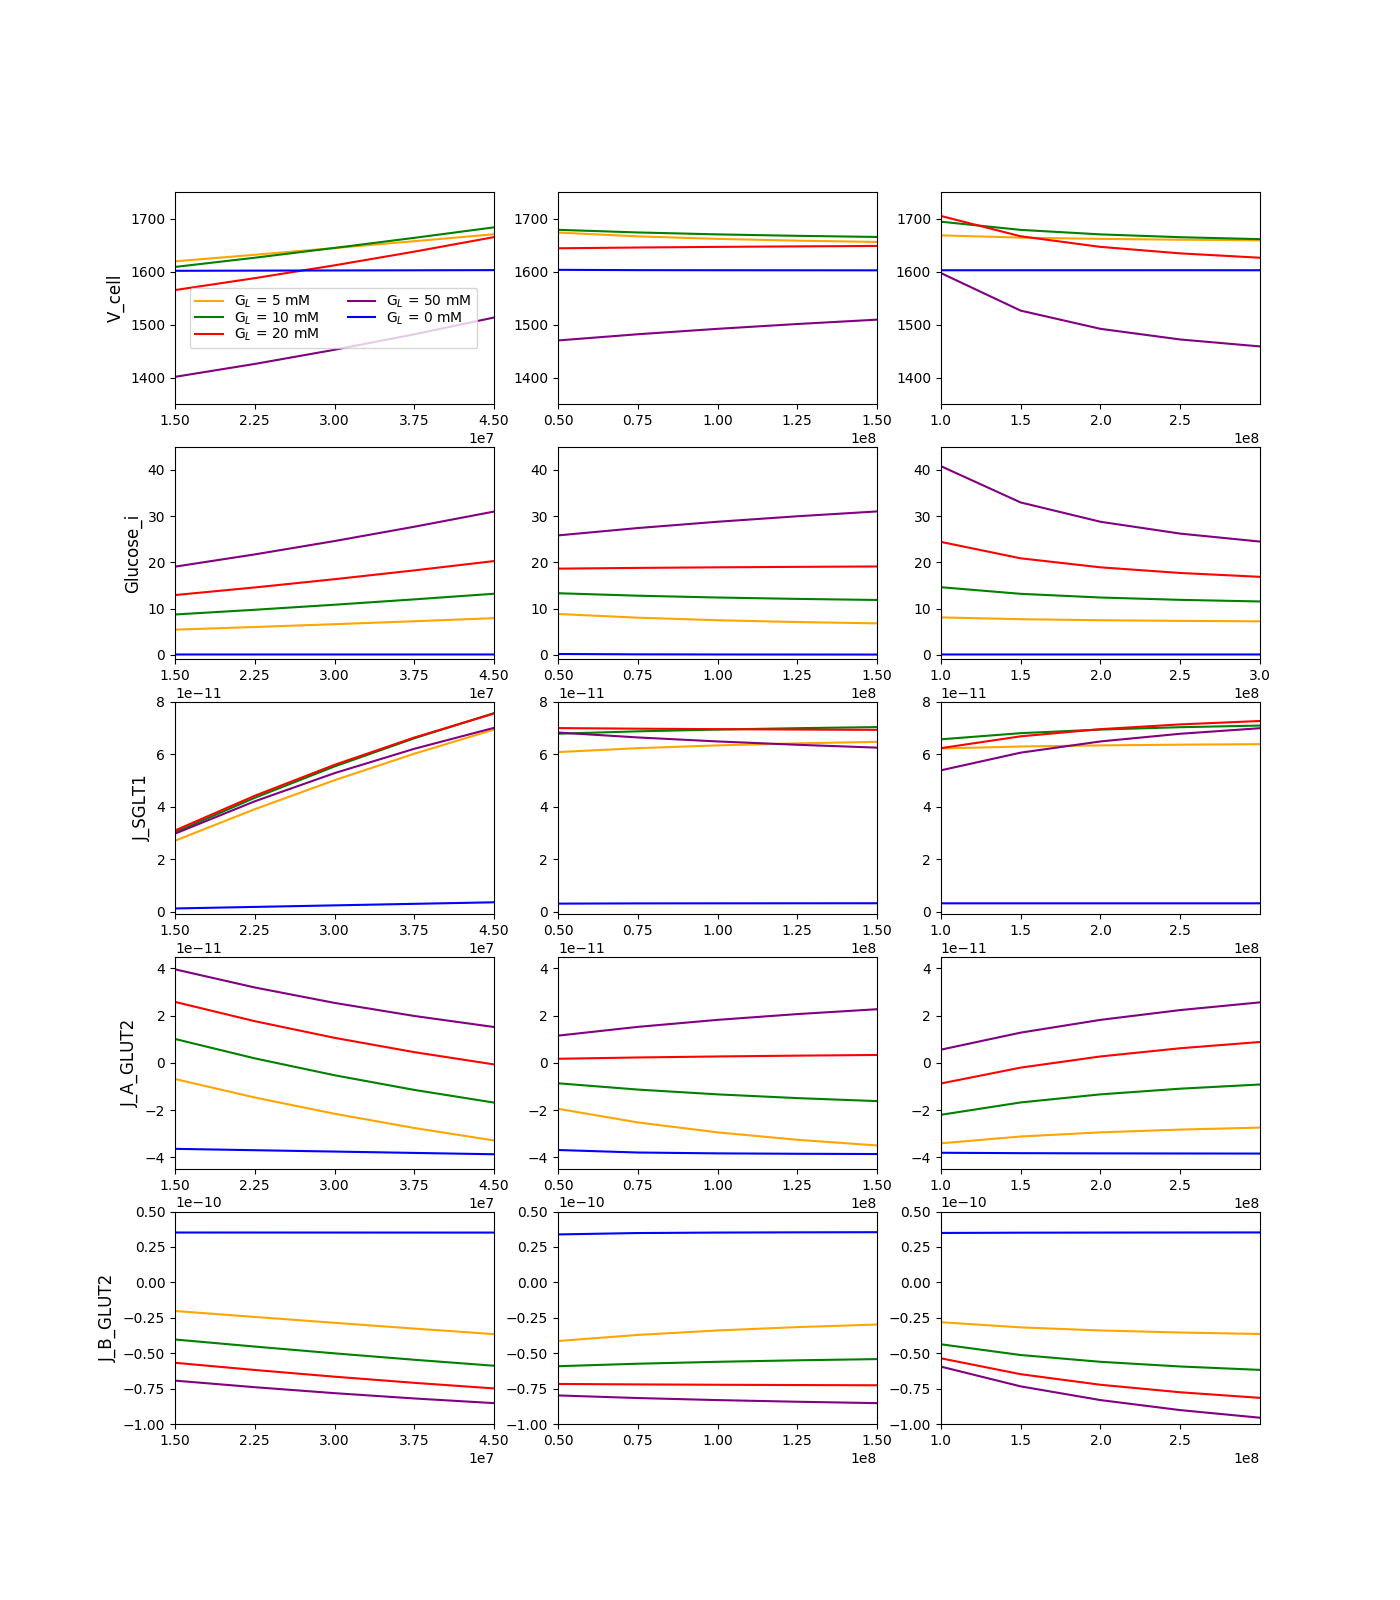
\includegraphics[width=1\linewidth]{Figure04}
\caption{Model response to different transporter densities. (A–C) Cell volume; (D–F) intracellular glucose; (G–I) SGLT1 glucose flux; (J–L) apical GLUT2 flux; (M–O) basolateral GLUT2 flux. In each column, one transporter density is varied while the other two are held constant at the reference value [nSGLT1 $= 3\times10^7$, nGLUT2 (apical) $= 10^8$, nGLUT2 (basolateral) $= 2\times10^8$]. This figure corresponds to Figure 6 in the primary paper and can be reproduced using \href{https://models.physiomeproject.org/workspace/840/rawfile/bc7a5ac43ddbd15d234e66d8cb17df8388d80064/Figure04.py}{Figure04.py}.}
\label{Figure4}
\end{figure}

\begin{figure}[htb]
\centering
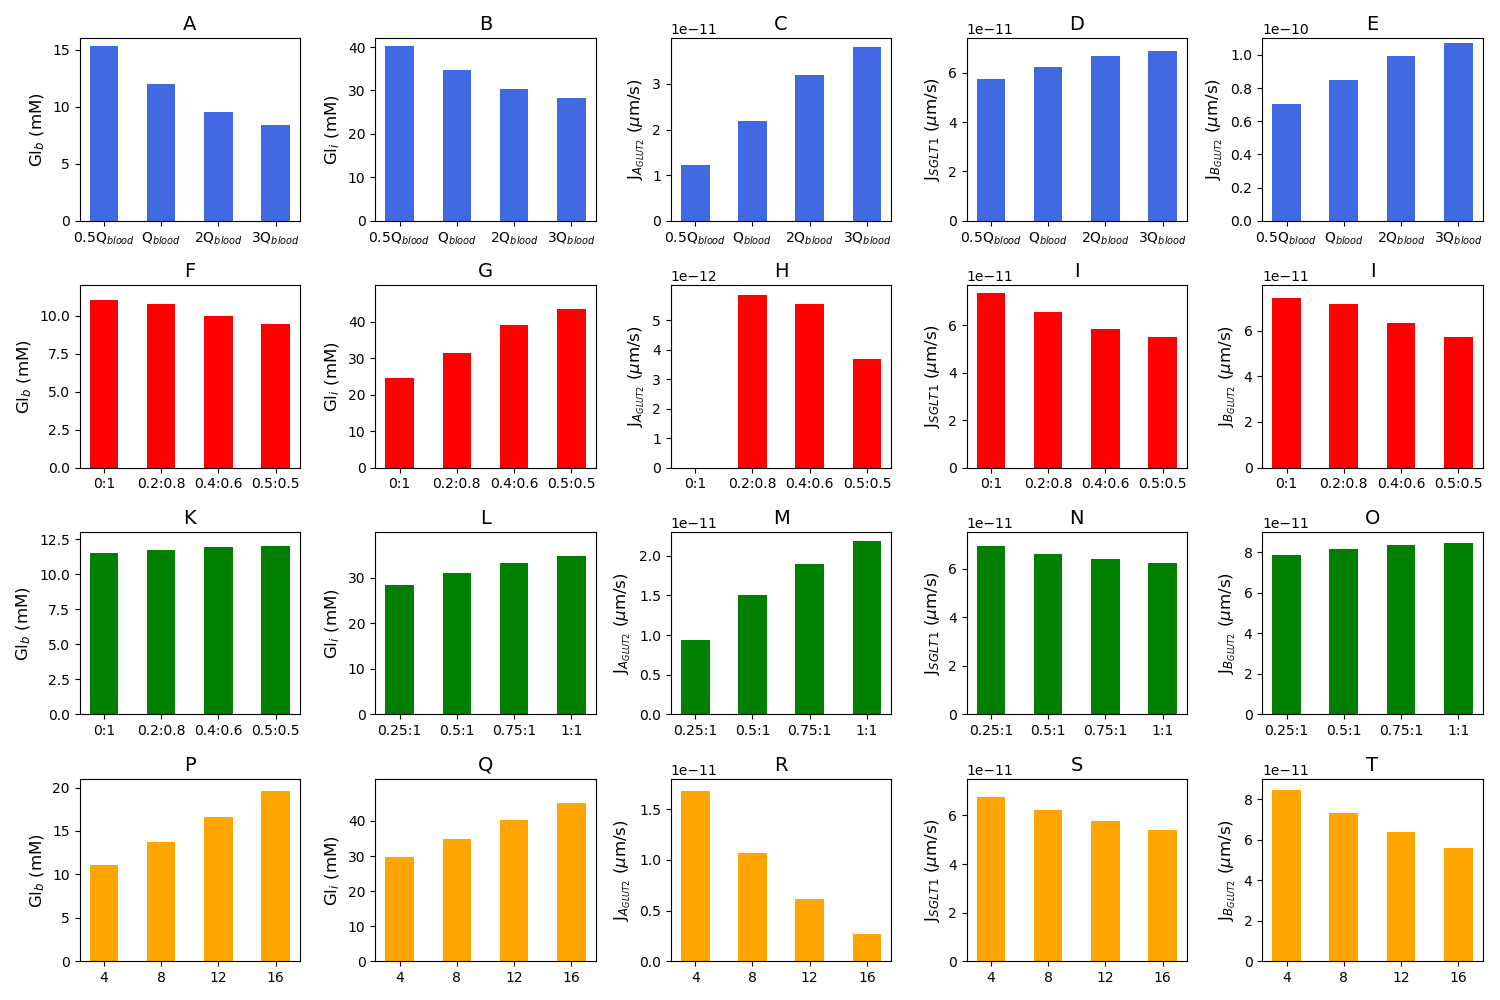
\includegraphics[width= 1\linewidth]{Figure05}
\caption{Blood glucose concentration, intracellular glucose concentration, apical GLUT2 flux, SGLT1 flux, and basolateral GLUT2 flux under different conditions. The first row is the model response to different blood flow rates. $Q_{blood}=10^{-17}$ m$^3$/s is the baseline value of the blood flow rate (A–E). The second row shows the response to variations in the inlet blood glucose concentration (F–J). Rows three and four consider two different scenarios for GLUT2 translocation to the apical membrane. Row three shows simulations run under the assumption that apical GLUT2 is translocated from basolateral GLUT2. Different ratios between apical and basolateral GLUT2 are considered with the total number fixed (K–O). Row four shows simulations run under the assumption that apical GLUT2 is translocated from intracellular vesicles. The number of basolateral GLUT2 is fixed and labels represent the fraction of total GLUT2 in the apical and basolateral membranes (P-T). This figure corresponds to Figure 7 in the primary paper and can be reproduced using \href{https://models.physiomeproject.org/workspace/840/rawfile/bc7a5ac43ddbd15d234e66d8cb17df8388d80064/Figure05.py}{Figure05.py}.}
\label{Figure5}
\end{figure}

\begin{figure}[htb]
\centering
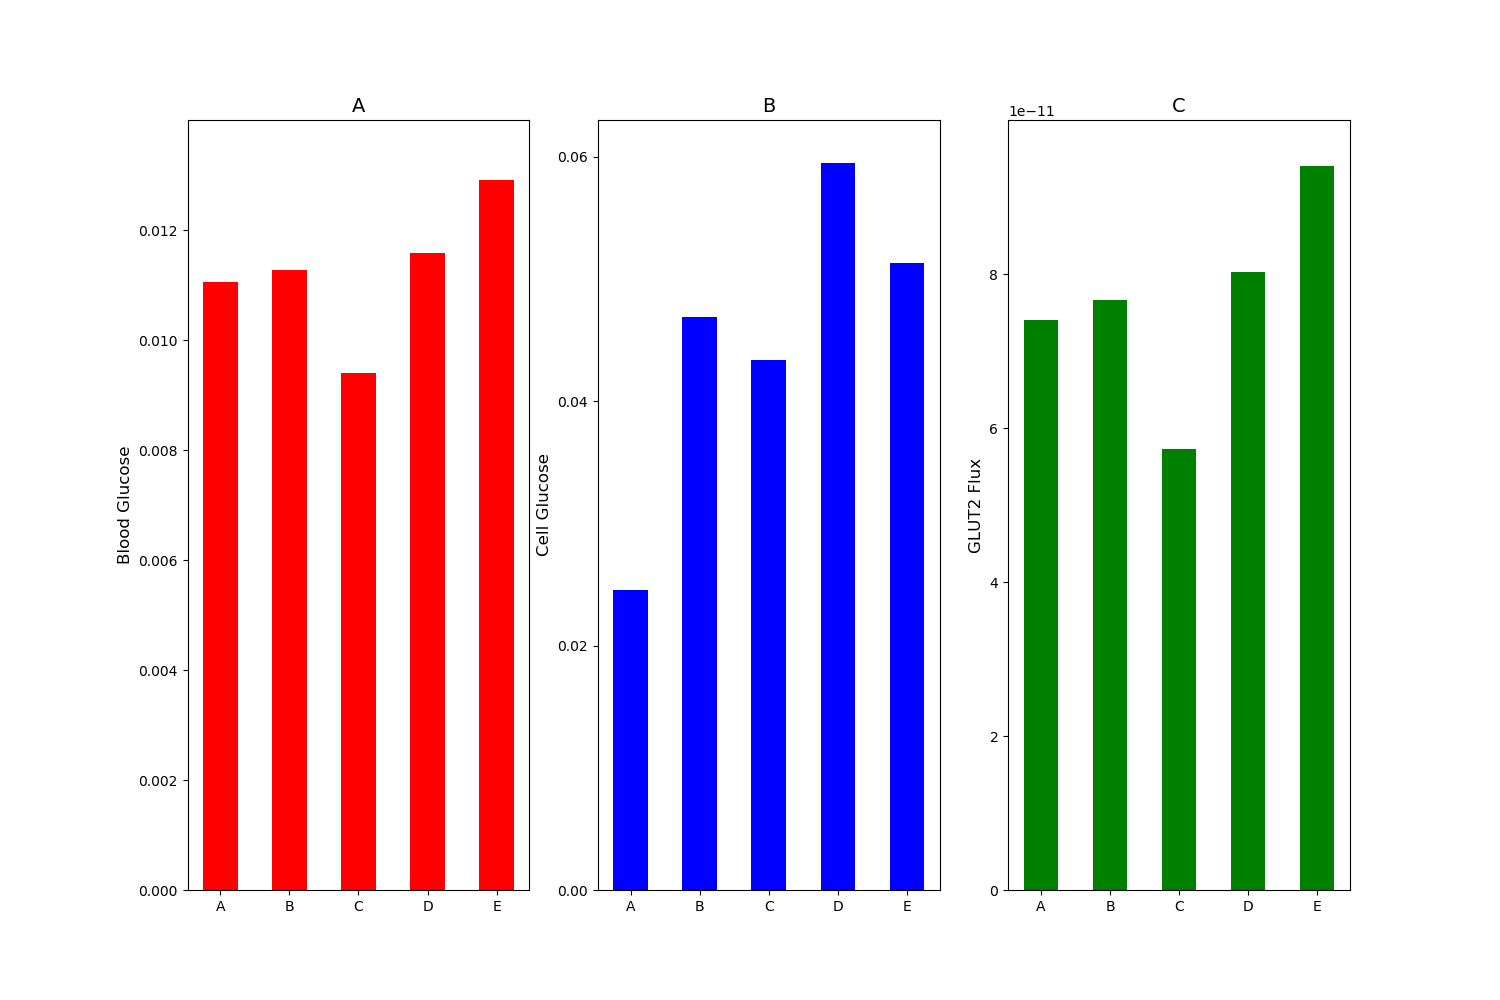
\includegraphics[width=0.9\linewidth]{Figure06}
\caption{(A) Blood glucose; (B) intracellular glucose; and (C) glucose flux into the blood. Simulation was run under $50$ mM stimulus of luminal glucose. Bar A: baseline with no apical GLUT2. Bar B: $50$\% increase in SGLT1 and apical GLUT2 equal to $0.5$ times basolateral GLUT2. Bar C: baseline SGLT1 and apical GLUT2 equal to $1.0$ times basolateral GLUT2. Bar D: $100$\% increase in SGLT1 and apical GLUT2 equal to $0.5$ times basolateral GLUT2. Bar E: $100$\% increase in SGLT1 alone with no apical GLUT2. This figure corresponds to Figure 8 in the primary paper and can be reproduced using \href{https://models.physiomeproject.org/workspace/840/rawfile/bc7a5ac43ddbd15d234e66d8cb17df8388d80064/Figure06.py}{Figure06.py}.}
\label{Figure6}
\end{figure}

\begin{figure}[htb]
\centering
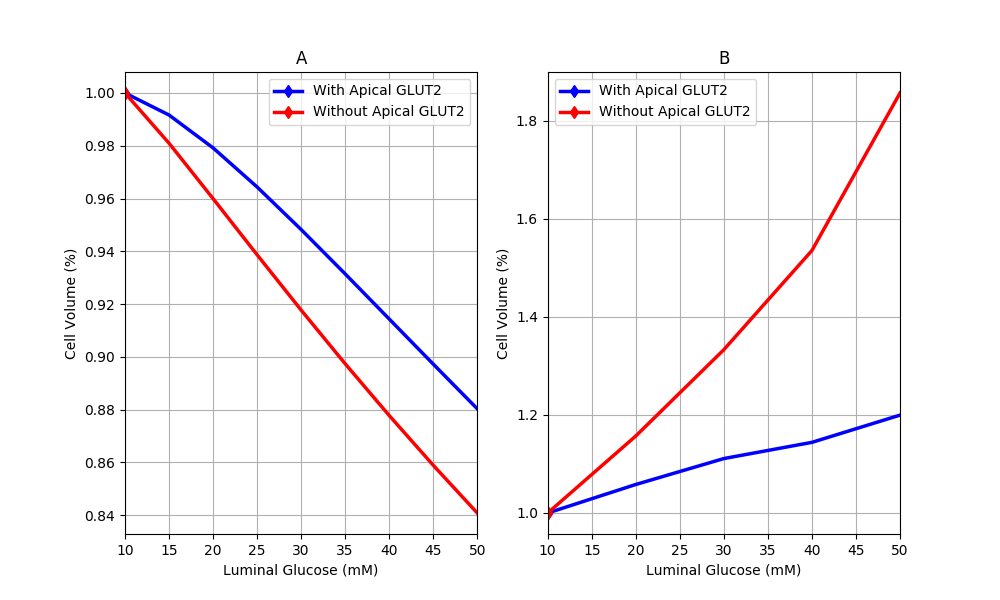
\includegraphics[width=0.9\linewidth]{Figure07}
\caption{Cell volume behaviour in response to different luminal glucose levels in (A) our model and (B) Naftalin's (2014) model. Values are normalised to baseline values. This figure corresponds to Figure 9 in the primary paper and can be reproduced using \href{https://models.physiomeproject.org/workspace/840/rawfile/bc7a5ac43ddbd15d234e66d8cb17df8388d80064/Figure07.py}{Figure07.py}.}
\label{Figure7}
\end{figure}

\section{Discussion}

In this manuscript, we used the CellML version of the cell model developed by \citet{afshar2021computational}. Most of the main figures in the primary article were reproducible using the CellML code provided by the authors. Some Python code was required and can be found in \url{https://models.physiomeproject.org/workspace/840}.\newline

\bibliography{references.bib}

\end{document}